\documentclass{article}
\usepackage{geometry}
\usepackage{graphicx}
\geometry{margin=1in}
\usepackage{amsmath}
\usepackage[english]{babel}
\usepackage[ruled,linesnumbered]{algorithm2e}
\usepackage{caption}
\usepackage{subcaption}

\title{}
\author{}

\begin{document}

\section{Deterministic Environment: Exploration Rate (Q-learning)}
\begin{figure}[h]
\subsection{Epsilon: 0.1}
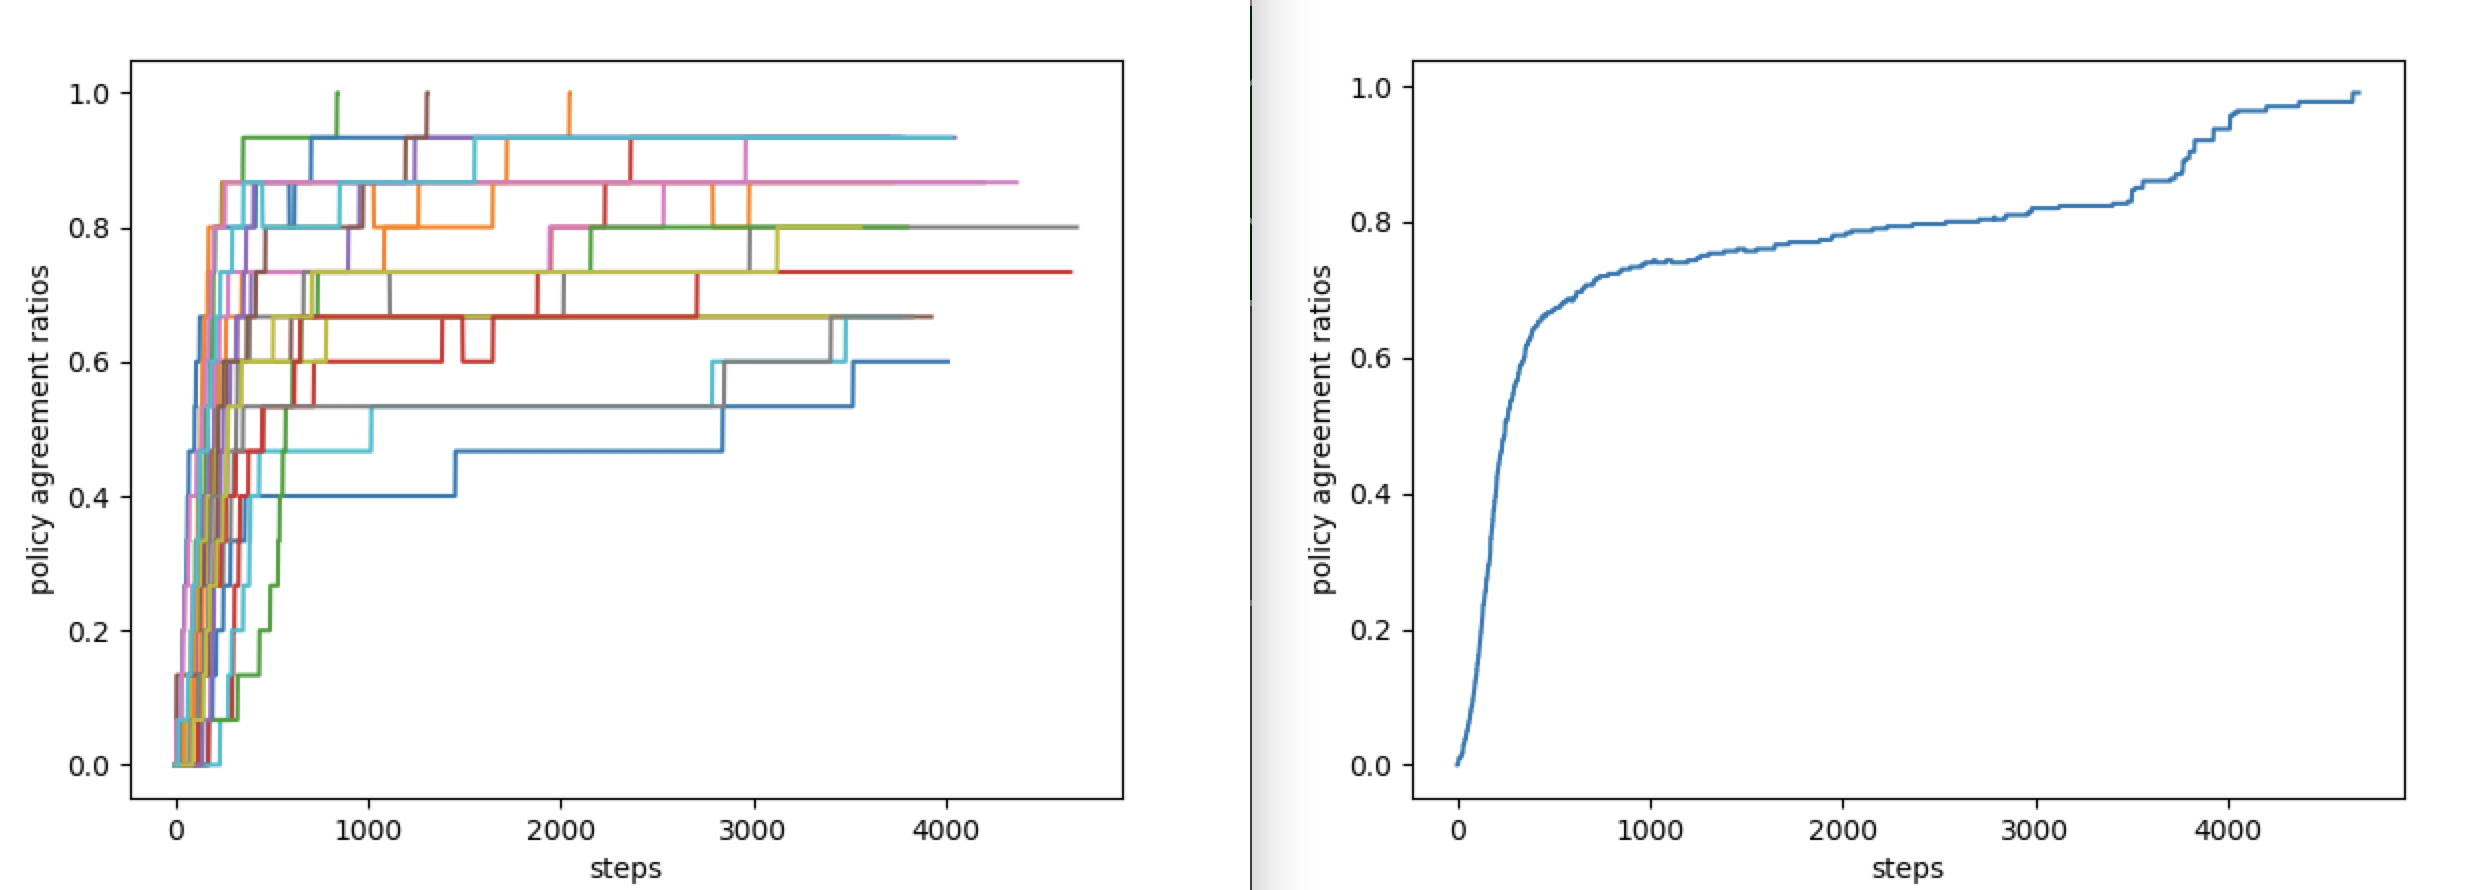
\includegraphics[width=0.9\linewidth, height=5cm]{images/epsilon_01.png} 
\caption{Deterministic Environment - Epsilon: 0.1 (Q-learning)}
\end{figure}

\subsection{Epsilon: 0.05}
\begin{figure}[h]
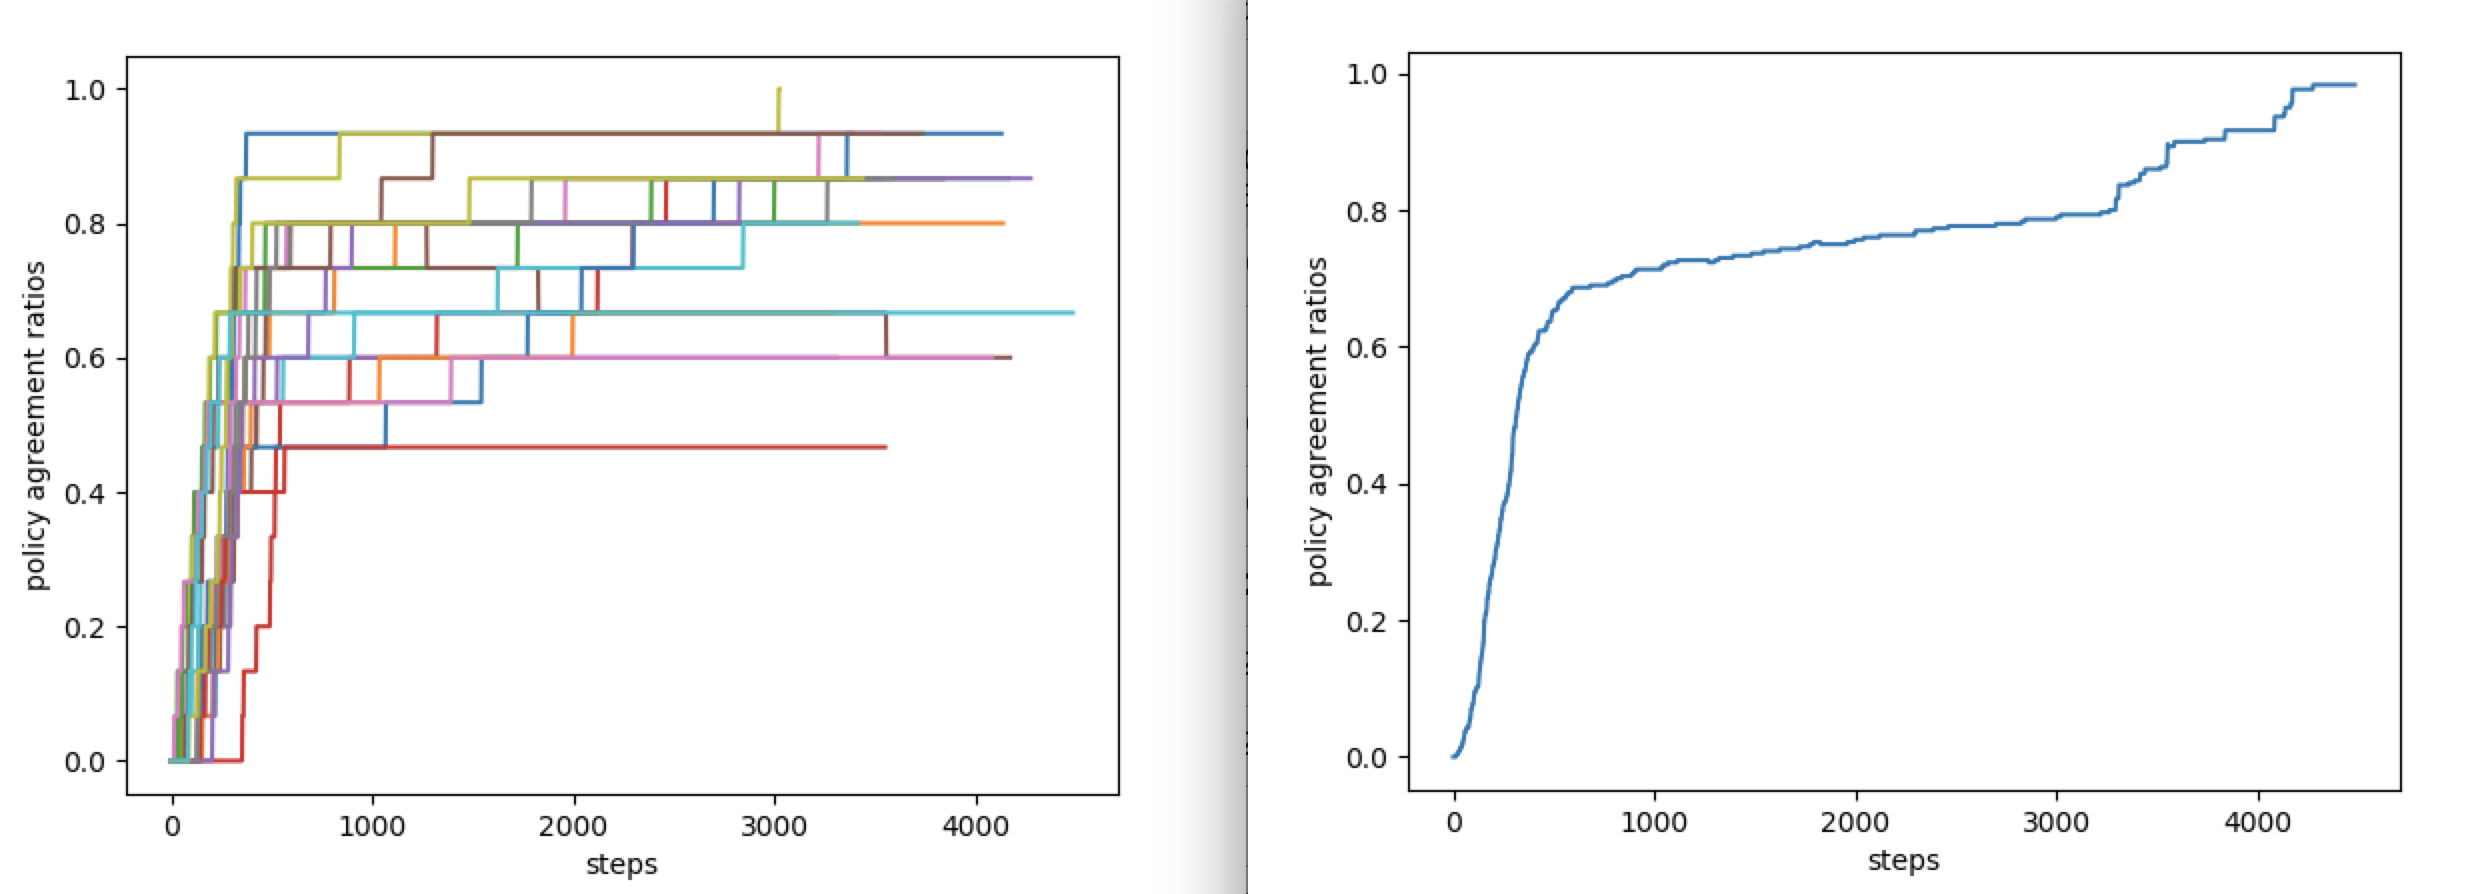
\includegraphics[width=0.9\linewidth, height=5cm]{images/epsilon_005.png} 
\caption{Deterministic Environment - Epsilon: 0.05 (Q-learning)}
\end{figure}


\subsection{Comparison}
\begin{figure}[h]
	\begin{subfigure}{0.5\textwidth}
		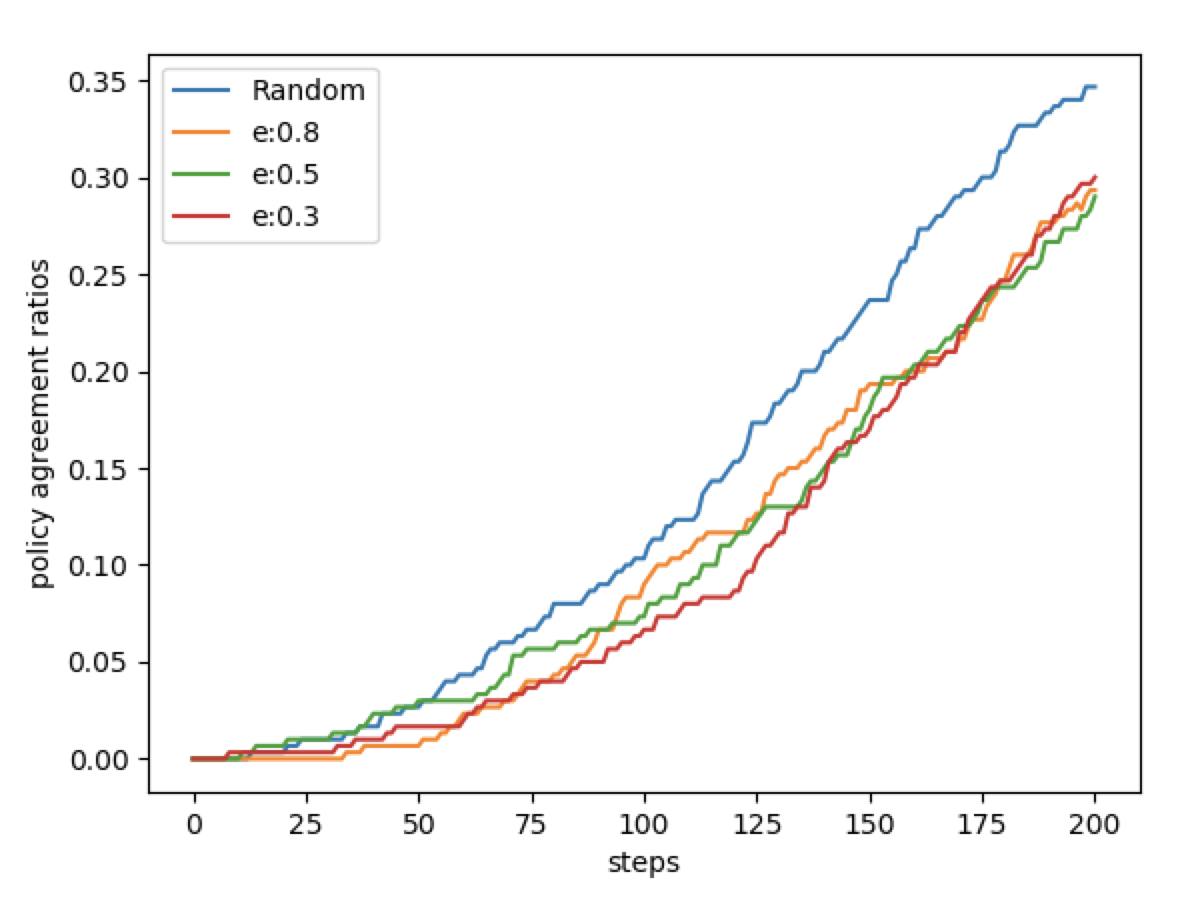
\includegraphics[width=0.9\linewidth, height=5cm]{images/epsilon_0_200.png} 
		\caption{}
	\end{subfigure}
	\begin{subfigure}{0.5\textwidth}
		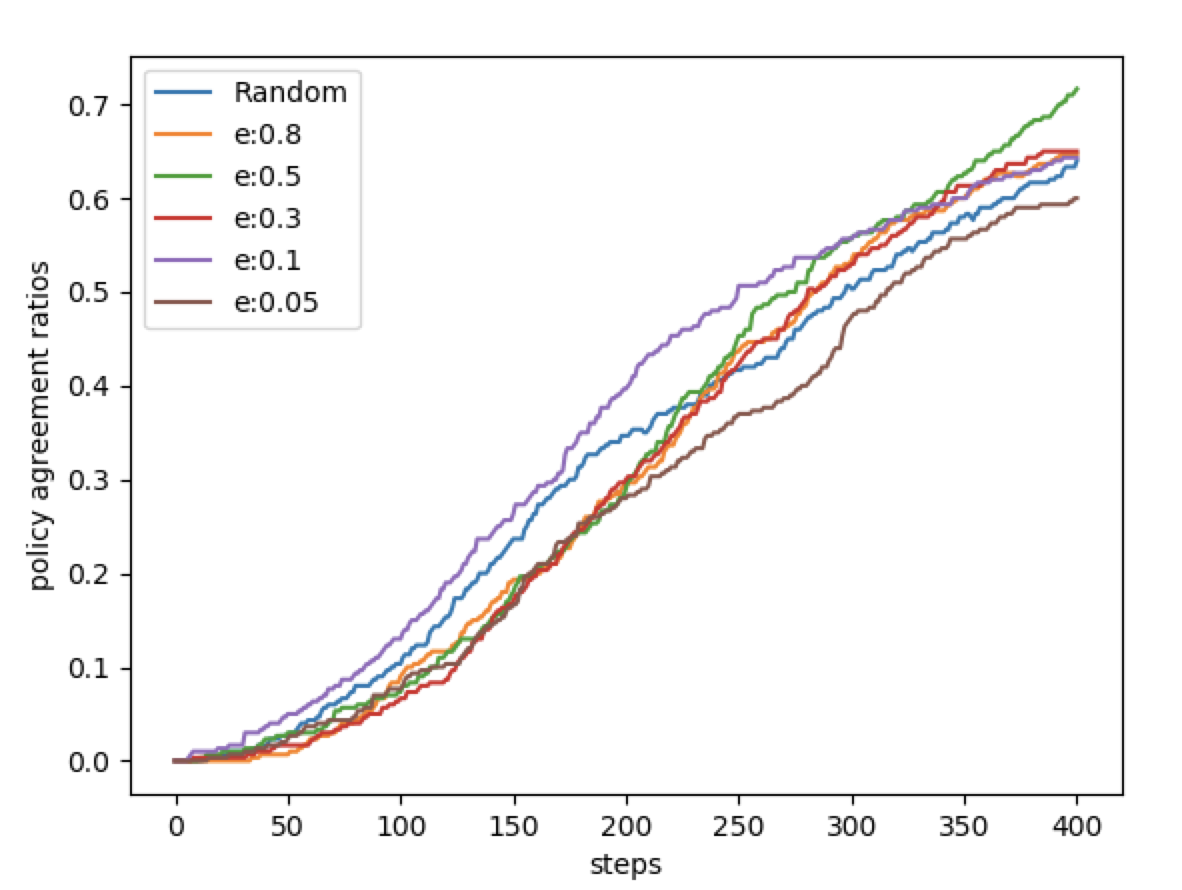
\includegraphics[width=0.9\linewidth, height=5cm]{images/epsilon_0_400.png}
		\caption{}
	\end{subfigure}
	\begin{subfigure}{0.5\textwidth}
		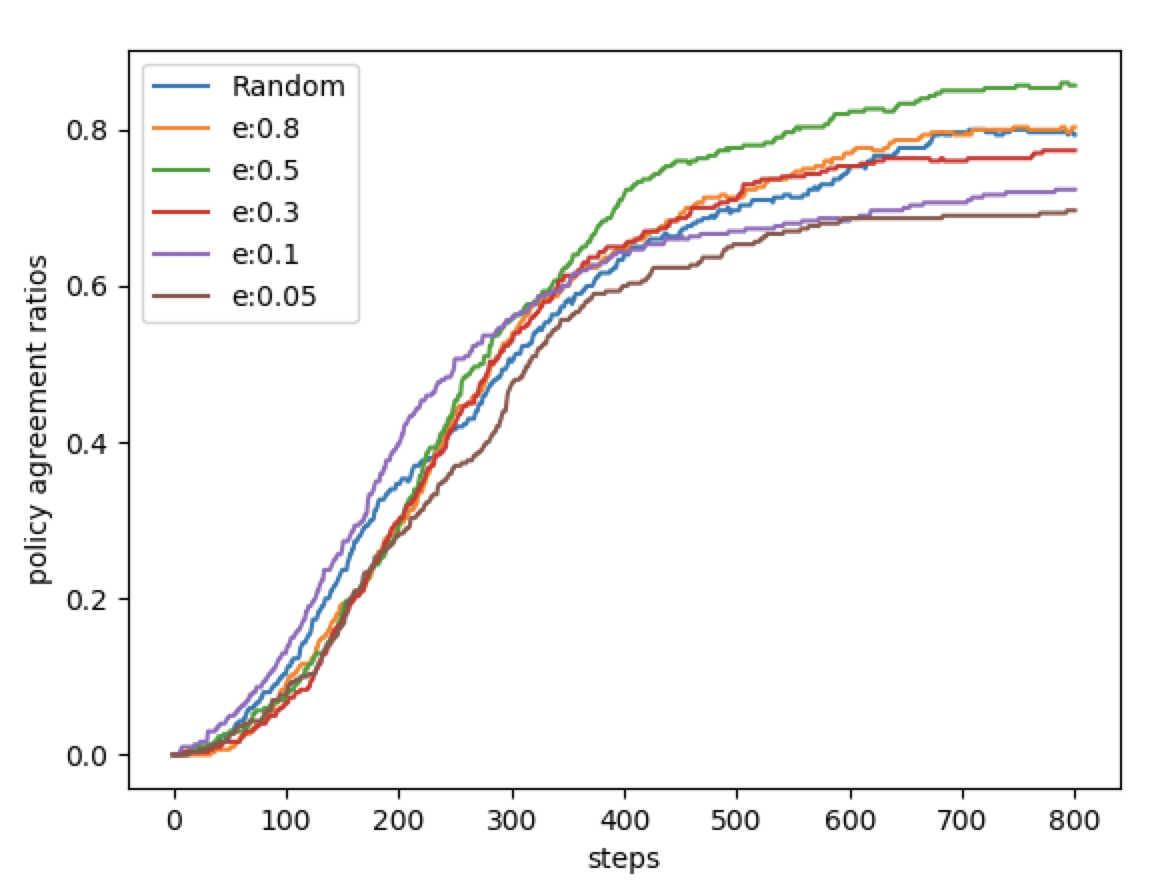
\includegraphics[width=0.9\linewidth, height=5cm]{images/epsilon_0_800.png}
		\caption{}
	\end{subfigure}
	\begin{subfigure}{0.5\textwidth}
		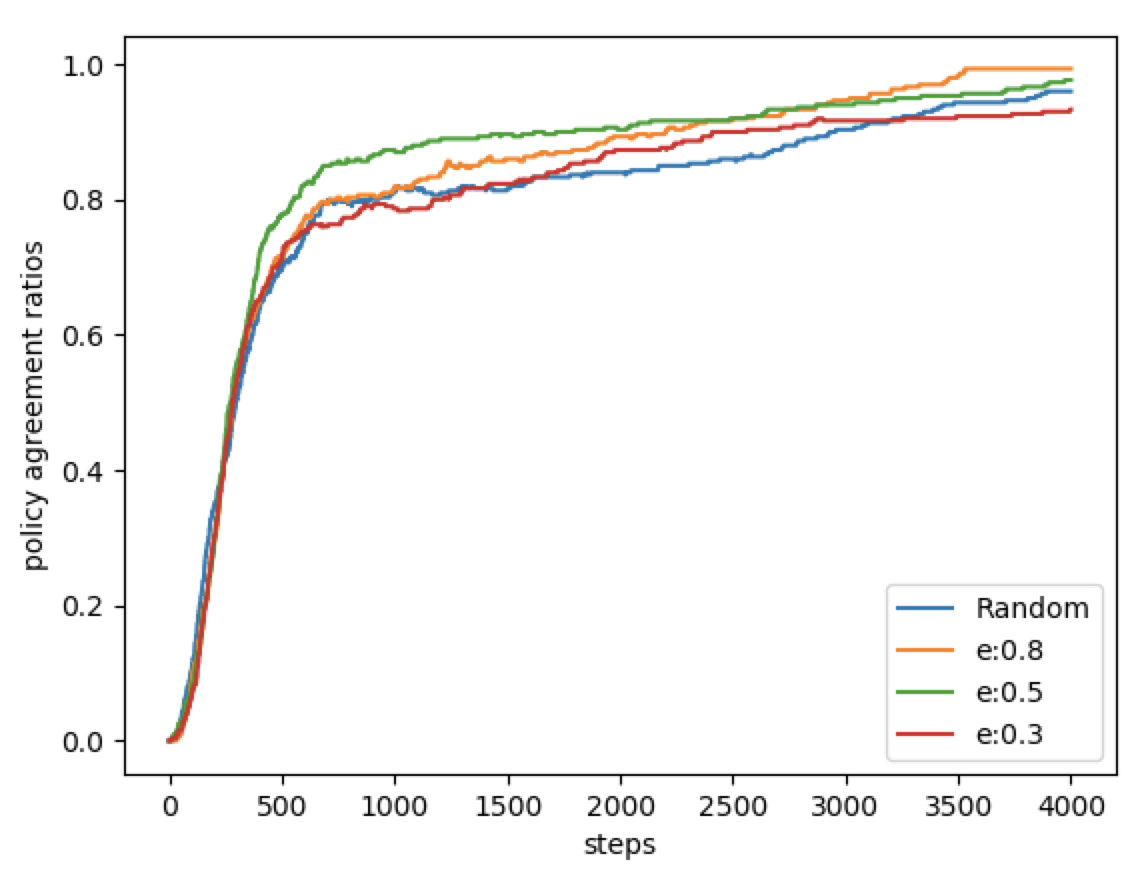
\includegraphics[width=0.9\linewidth, height=5cm]{images/epsilon_0_4000.png}
		\caption{}
	\end{subfigure}
	\caption{Average policy agreement ratios at each time step of experiments with different epsilon values. (Q-learning)}
\end{figure}

\section{TAMER using epsilon-greedy}
\begin{figure}[h]
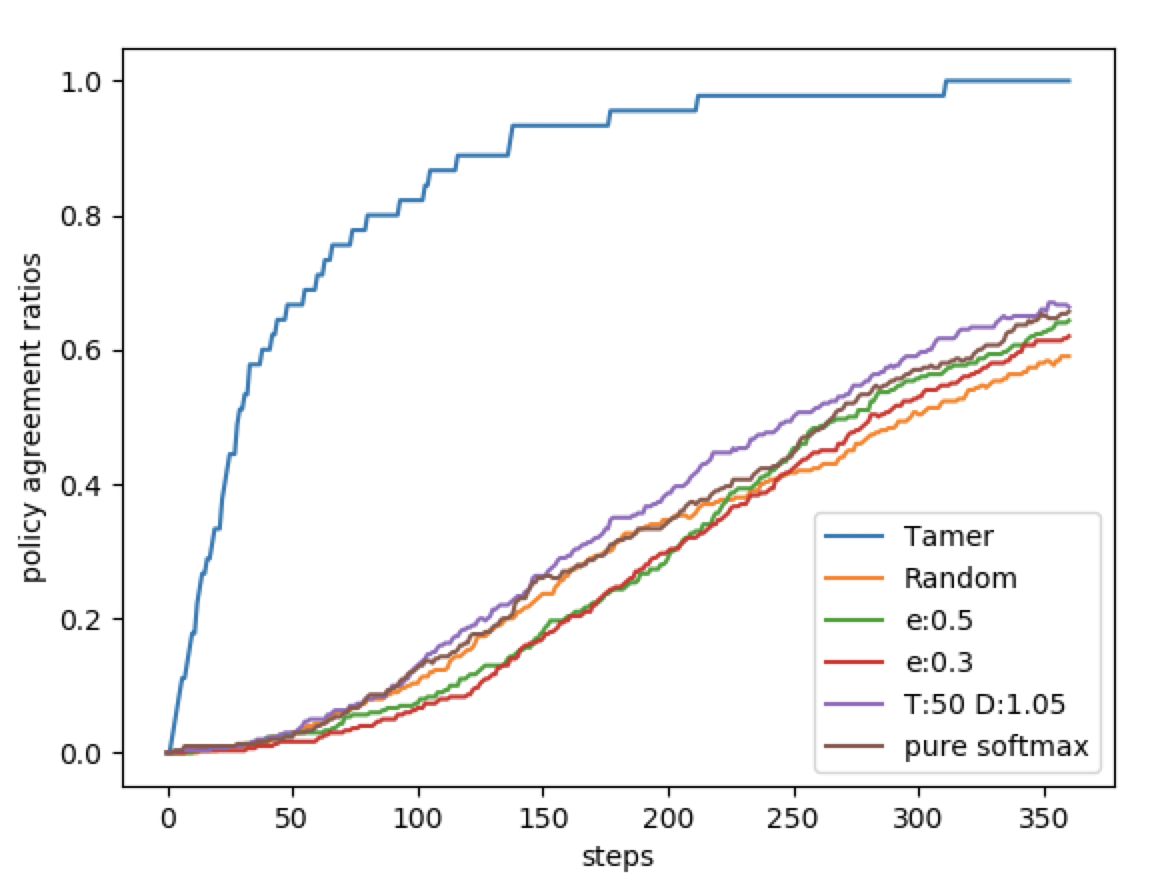
\includegraphics[width=15cm]{images/all_0_400.png} 
\caption{TAMER using epsilon-greedy. (TAMER)}
\end{figure}

\section{Noise: 0.1}
\begin{figure}[h]
	\begin{subfigure}{0.5\textwidth}
		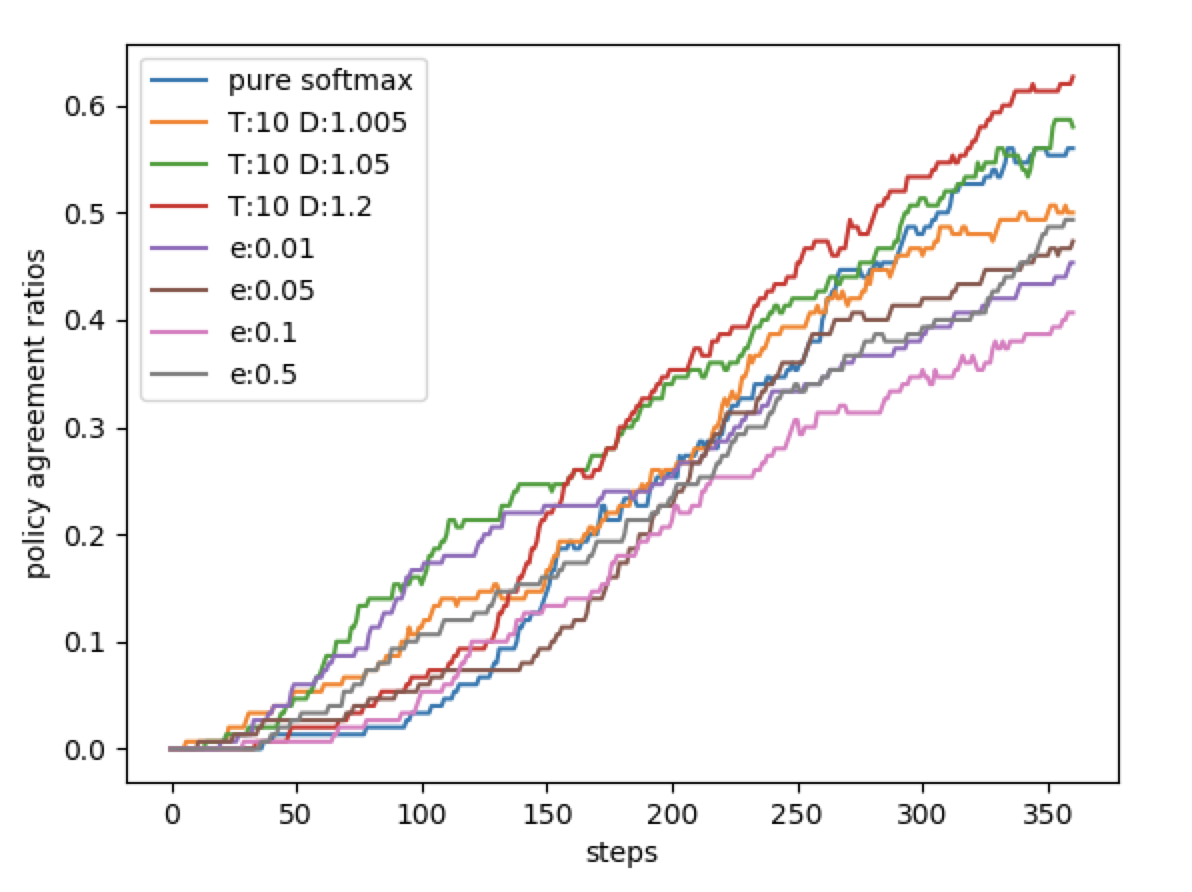
\includegraphics[width=0.9\linewidth, height=5cm]{images/noise01_400.png} 
		\caption{}
	\end{subfigure}
	\begin{subfigure}{0.5\textwidth}
		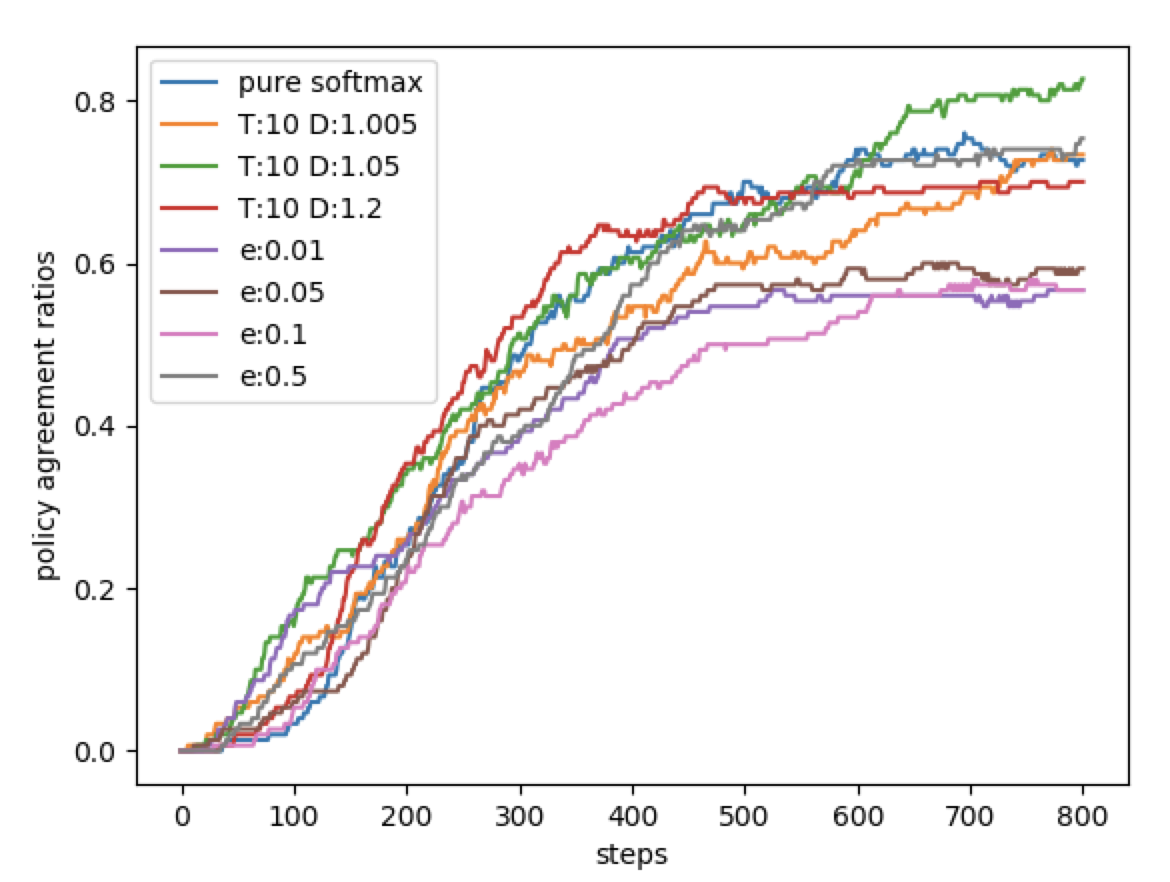
\includegraphics[width=0.9\linewidth, height=5cm]{images/noise01_800.png}
		\caption{}
	\end{subfigure}
	\begin{subfigure}{0.5\textwidth}
		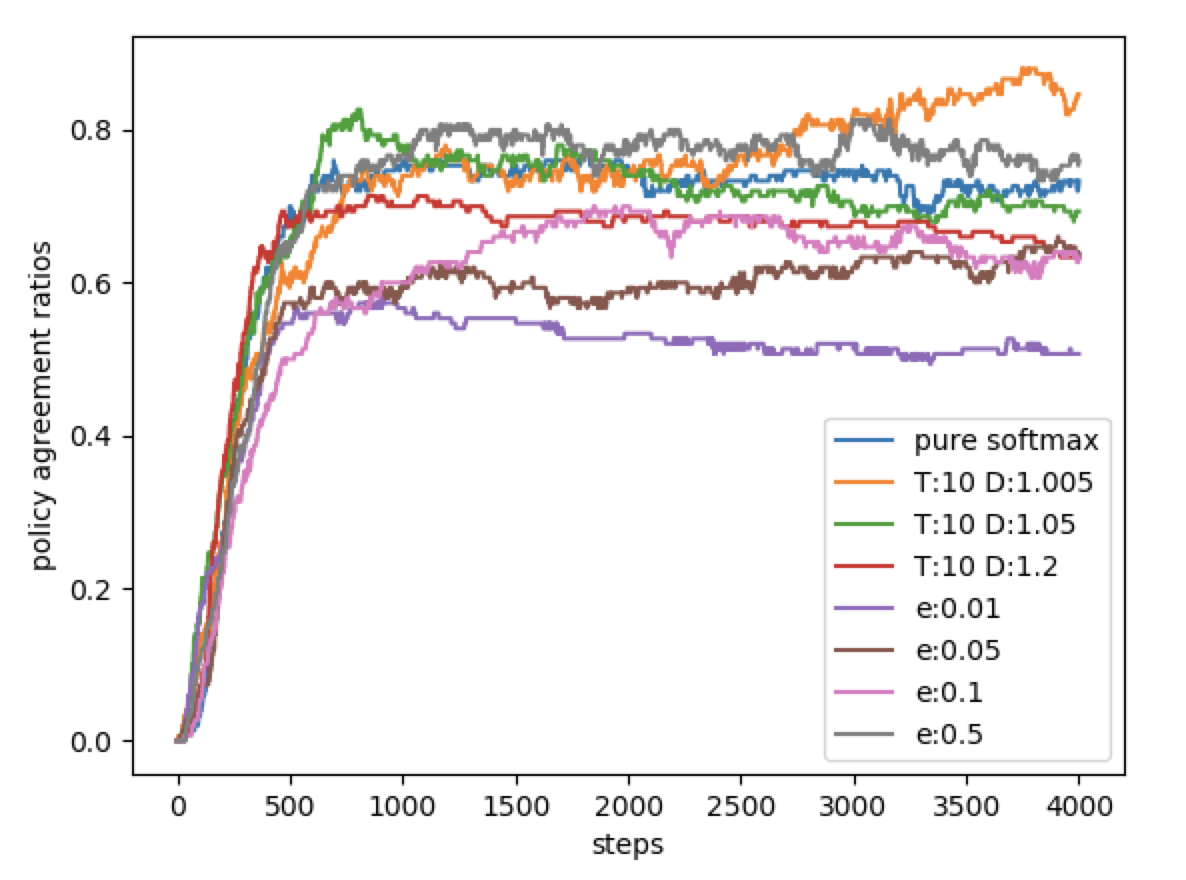
\includegraphics[width=0.9\linewidth, height=5cm]{images/noise01_4000.png}
		\caption{}
	\end{subfigure}
	\caption{Noise: 0.1}
\end{figure}

\section{Noise: 0.5}
\begin{figure}[h]
	\begin{subfigure}{0.5\textwidth}
		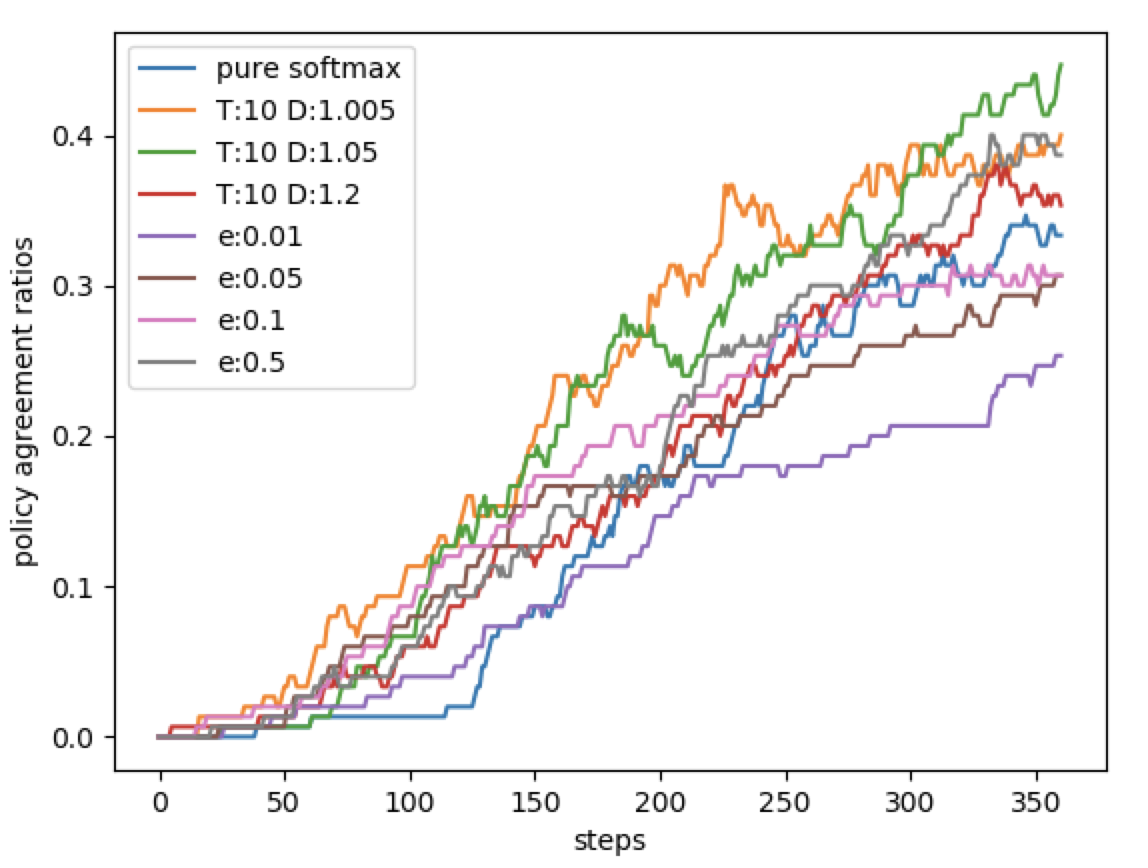
\includegraphics[width=0.9\linewidth, height=5cm]{images/noise05_400.png} 
		\caption{}
	\end{subfigure}
	\begin{subfigure}{0.5\textwidth}
		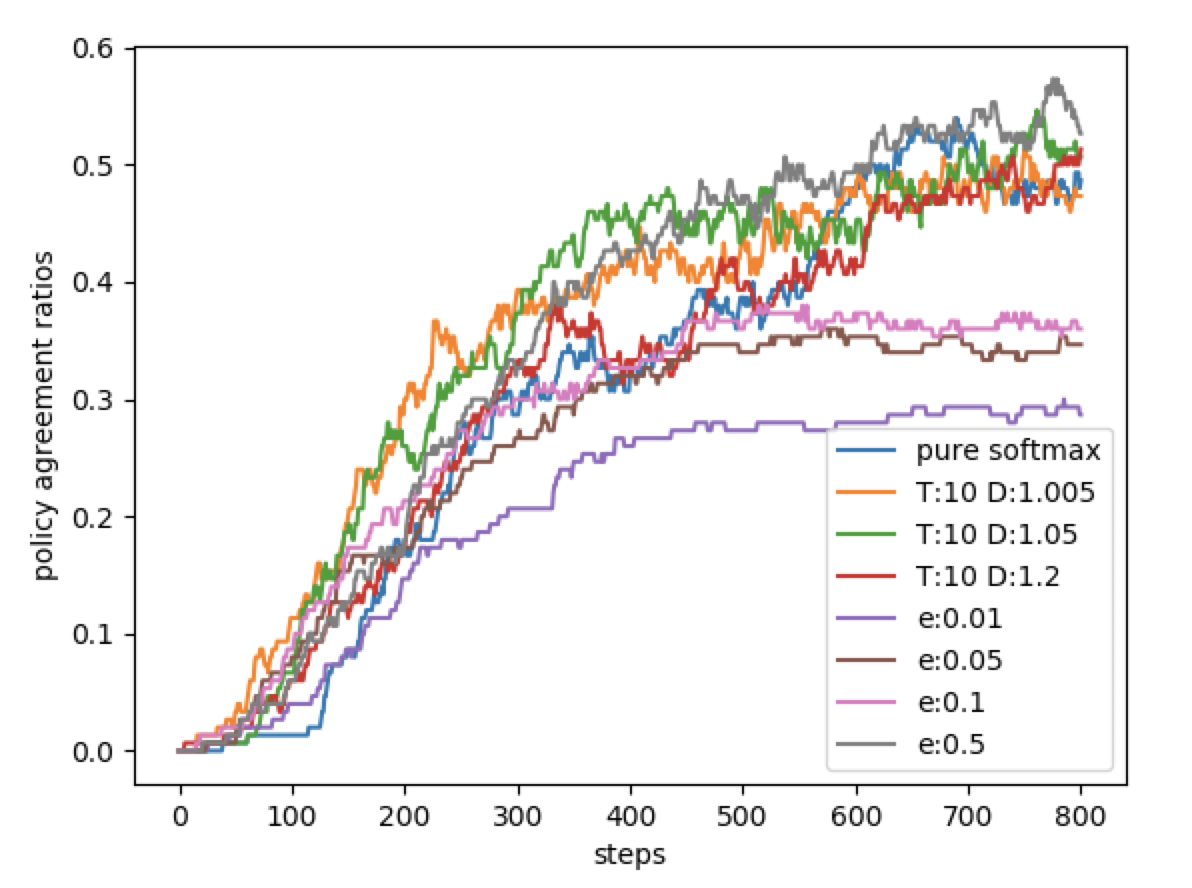
\includegraphics[width=0.9\linewidth, height=5cm]{images/noise05_800.png}
		\caption{}
	\end{subfigure}
	\begin{subfigure}{0.5\textwidth}
		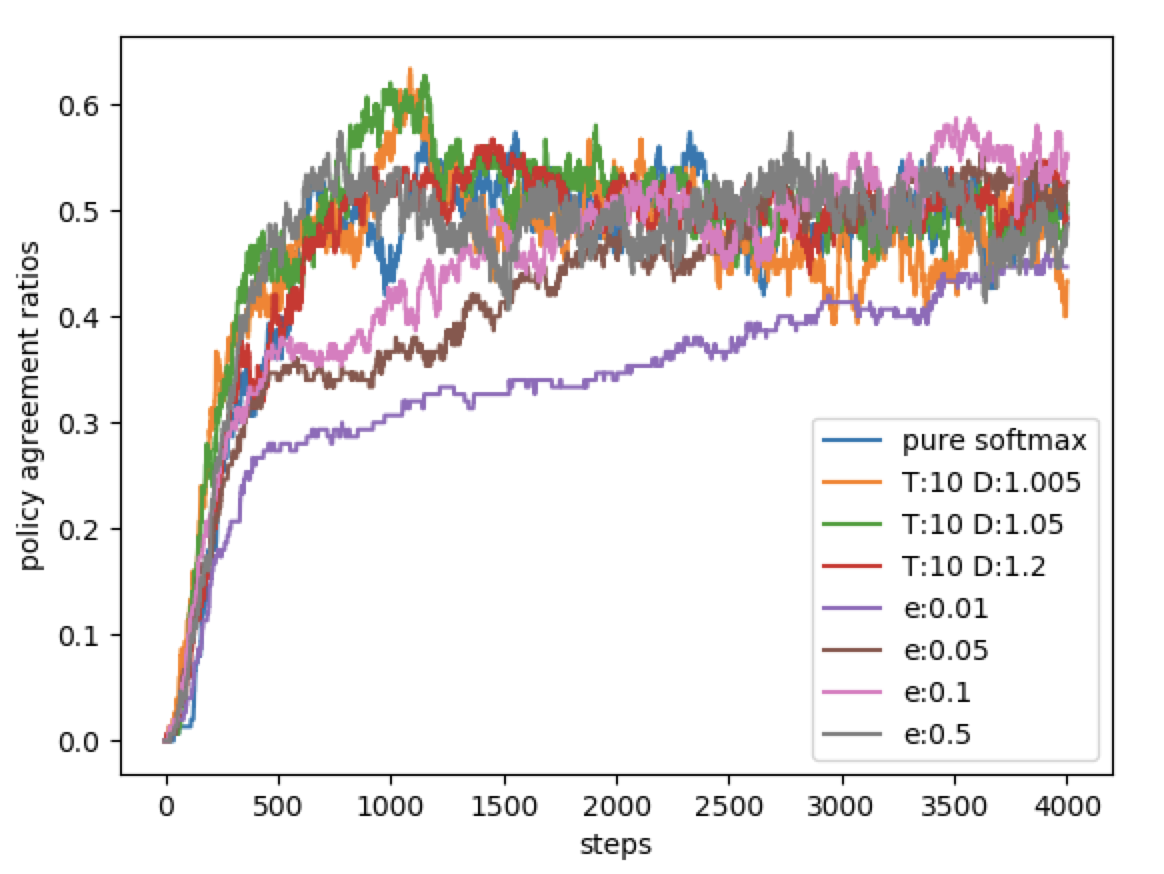
\includegraphics[width=0.9\linewidth, height=5cm]{images/noise05_4000.png}
		\caption{}
	\end{subfigure}
	\begin{subfigure}{0.5\textwidth}
		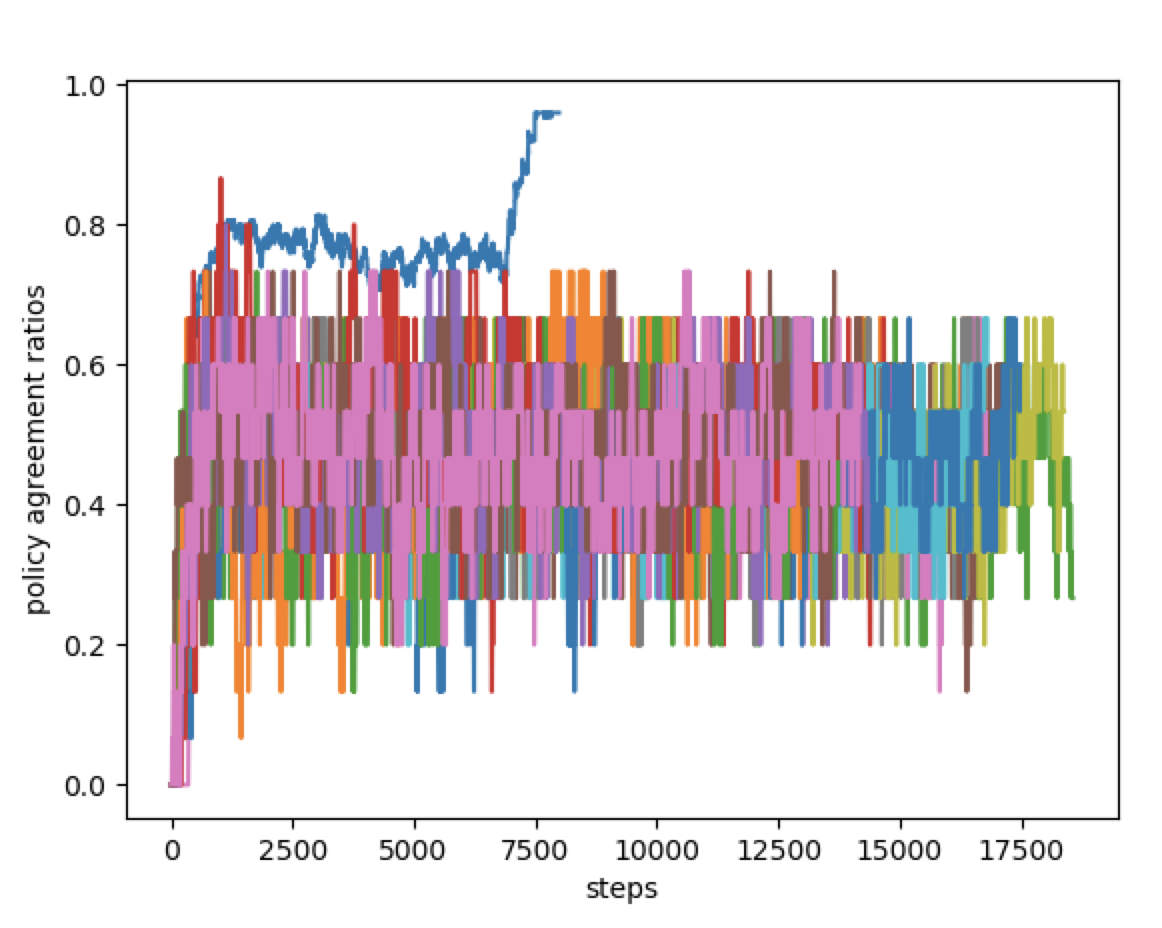
\includegraphics[width=0.9\linewidth, height=5cm]{images/noise05_unstable.png}
		\caption{}
	\end{subfigure}
	\caption{Noise: 0.5}
\end{figure}

\section{Noise: 0.9}
\begin{figure}[h]
	\begin{subfigure}{0.5\textwidth}
		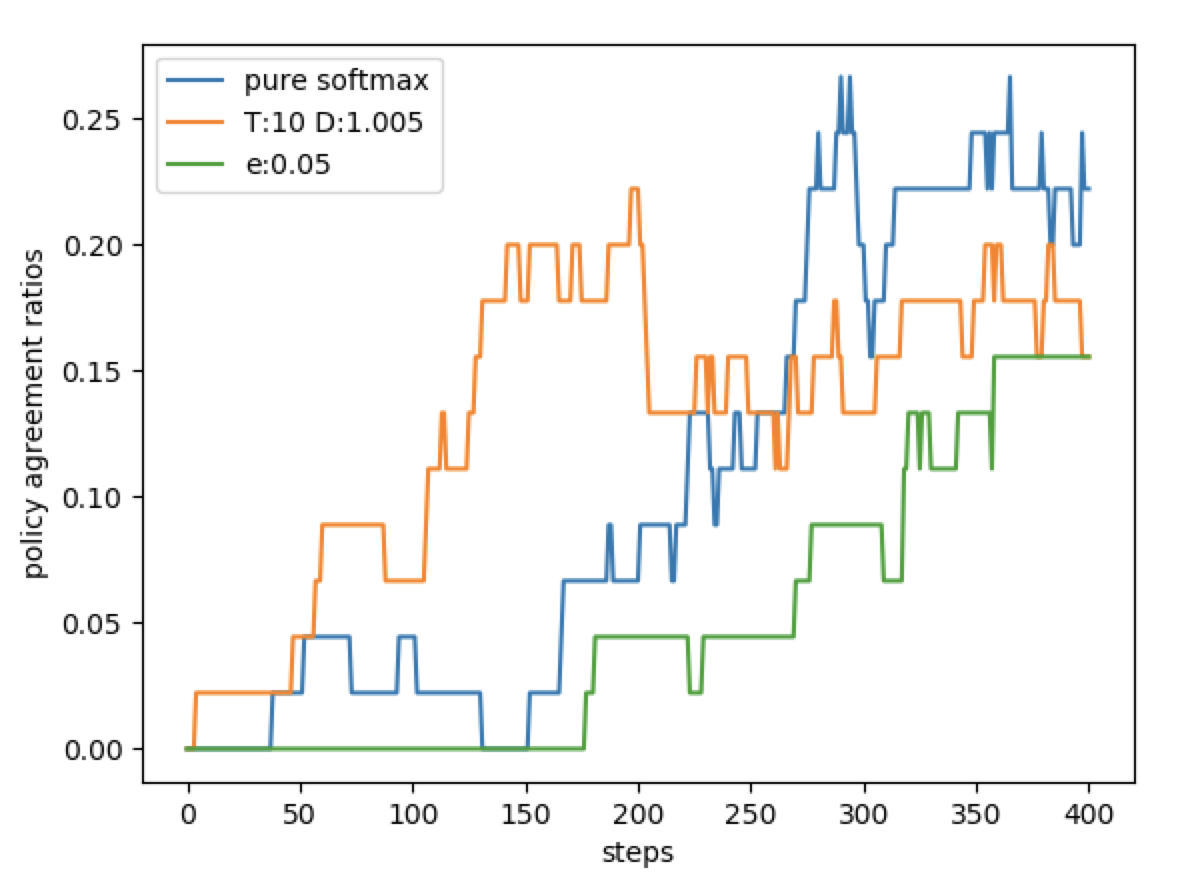
\includegraphics[width=0.9\linewidth, height=5cm]{images/noise09_400.png} 
		\caption{}
	\end{subfigure}
	\begin{subfigure}{0.5\textwidth}
		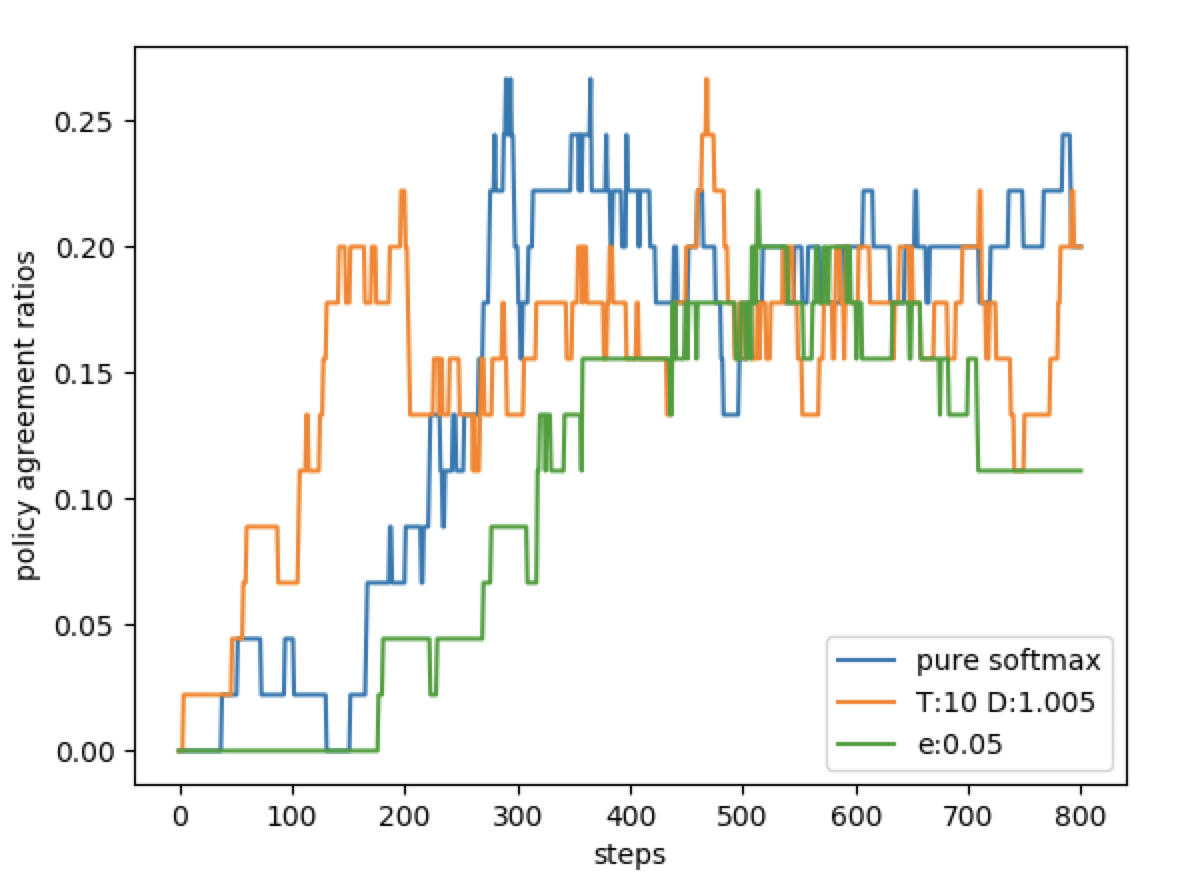
\includegraphics[width=0.9\linewidth, height=5cm]{images/noise09_800.png}
		\caption{}
	\end{subfigure}
	\begin{subfigure}{0.5\textwidth}
		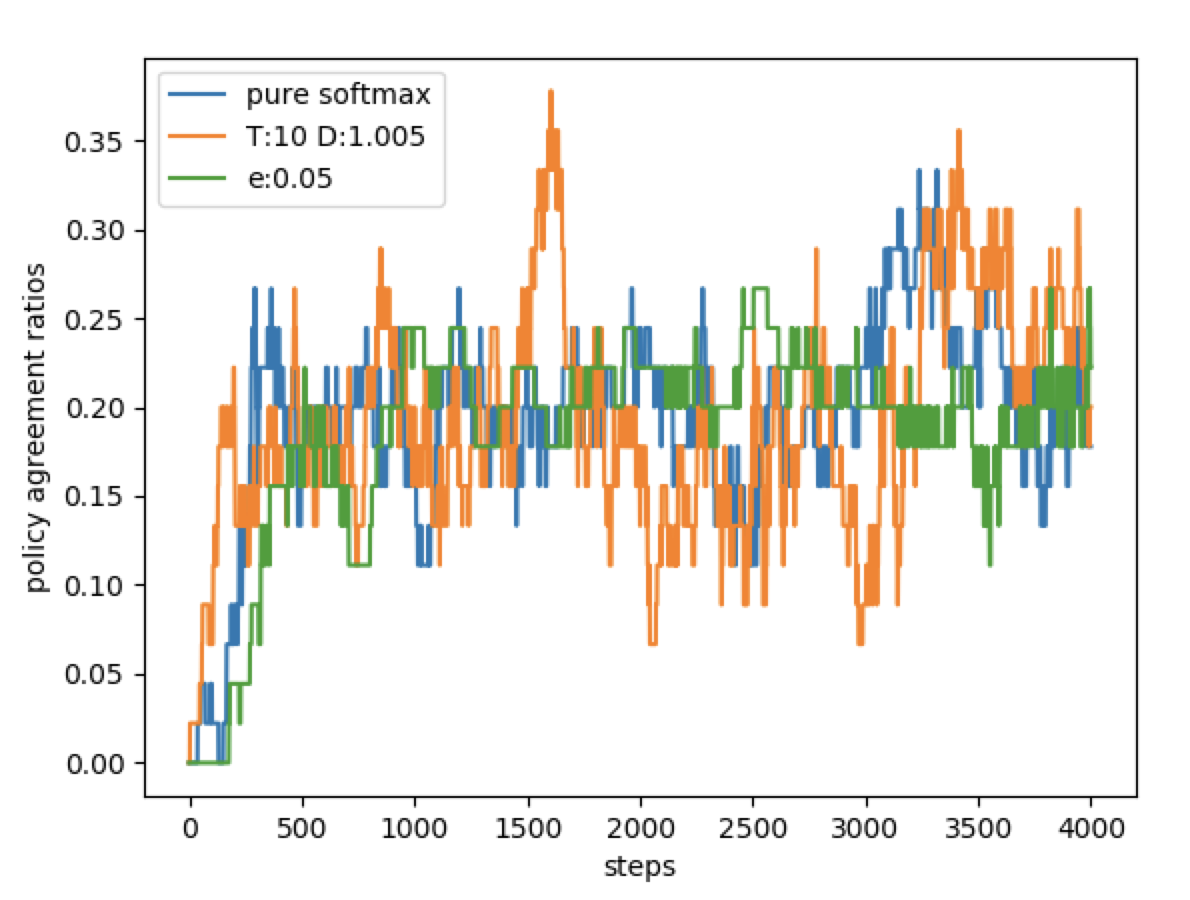
\includegraphics[width=0.9\linewidth, height=5cm]{images/noise09_4000.png}
		\caption{}
	\end{subfigure}
	\caption{Noise: 0.9}
\end{figure}

\section{Different Learning Rate with Noise 0.2}
\begin{figure}[h]
	\begin{subfigure}{0.5\textwidth}
		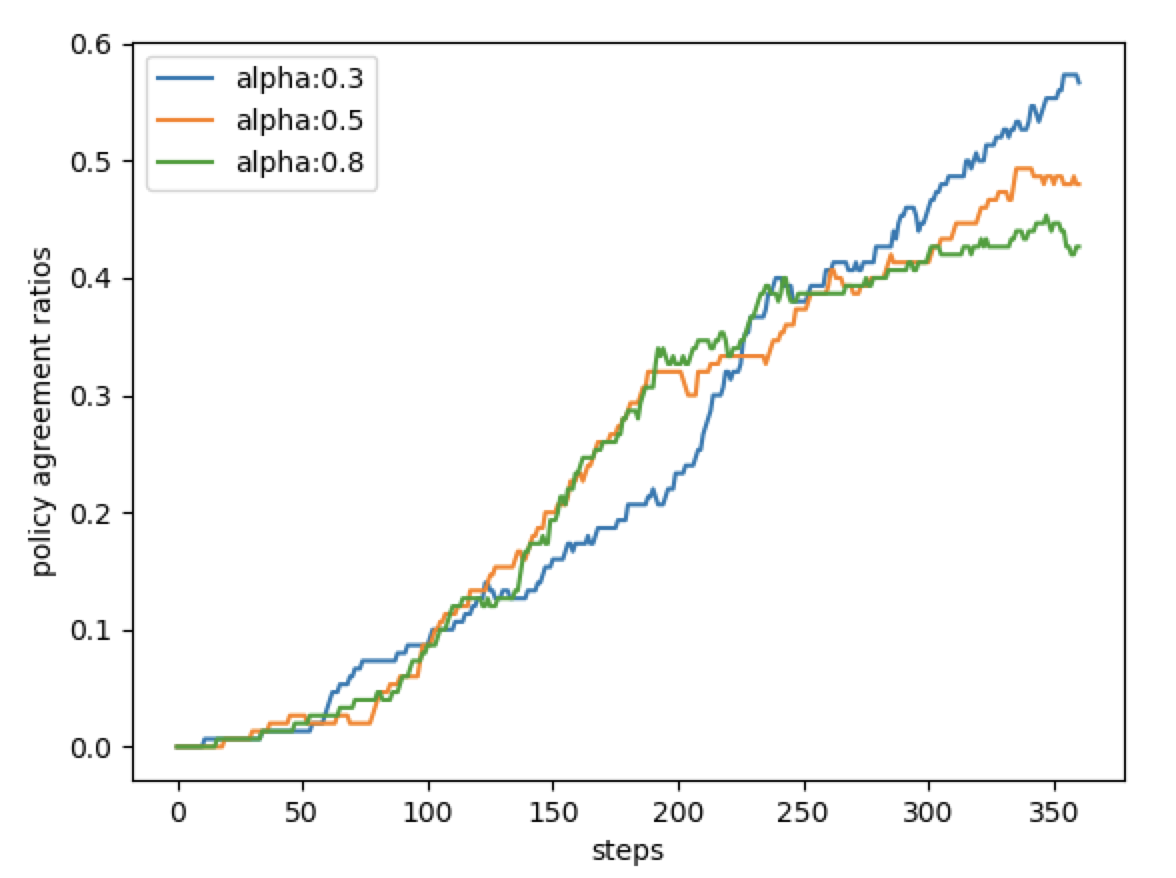
\includegraphics[width=0.9\linewidth, height=5cm]{images/alpha_noise02_400.png} 
		\caption{}
	\end{subfigure}
	\begin{subfigure}{0.5\textwidth}
		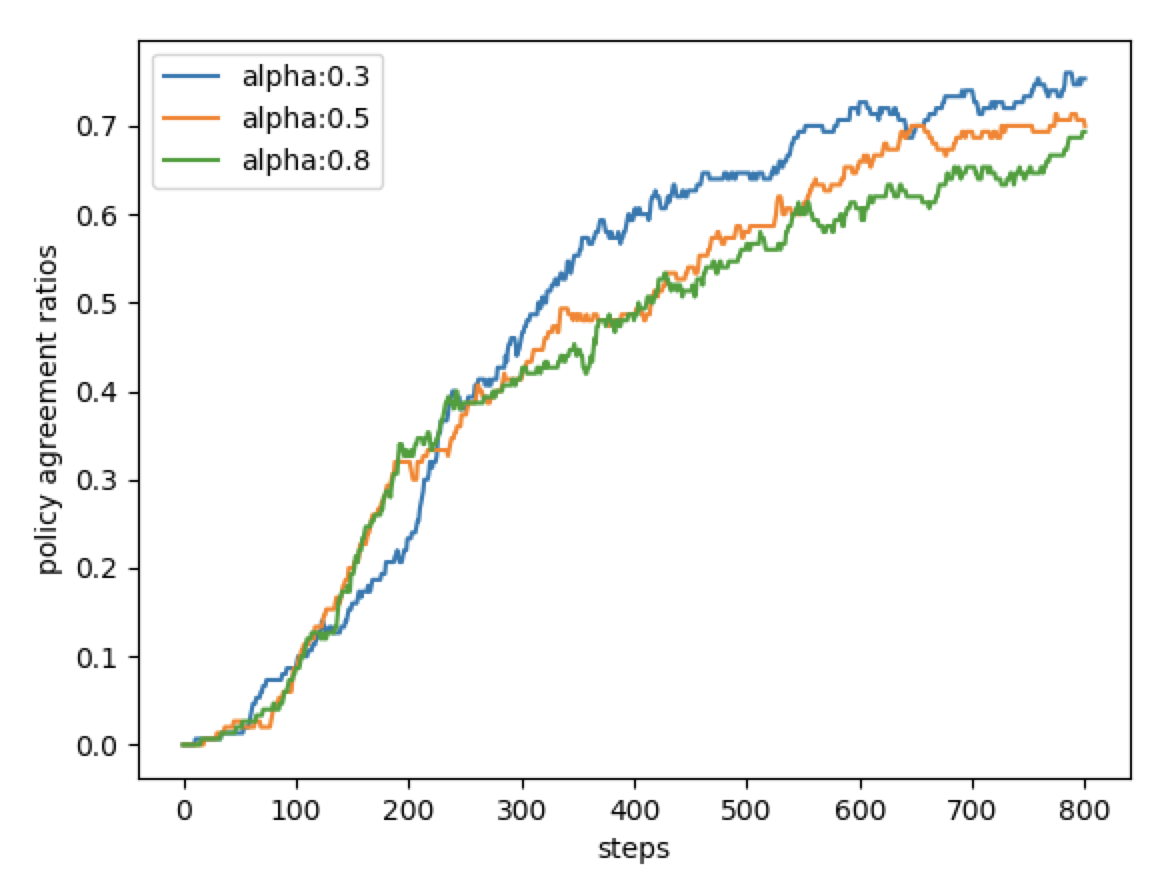
\includegraphics[width=0.9\linewidth, height=5cm]{images/alpha_noise02_800.png}
		\caption{}
	\end{subfigure}
	\begin{subfigure}{0.5\textwidth}
		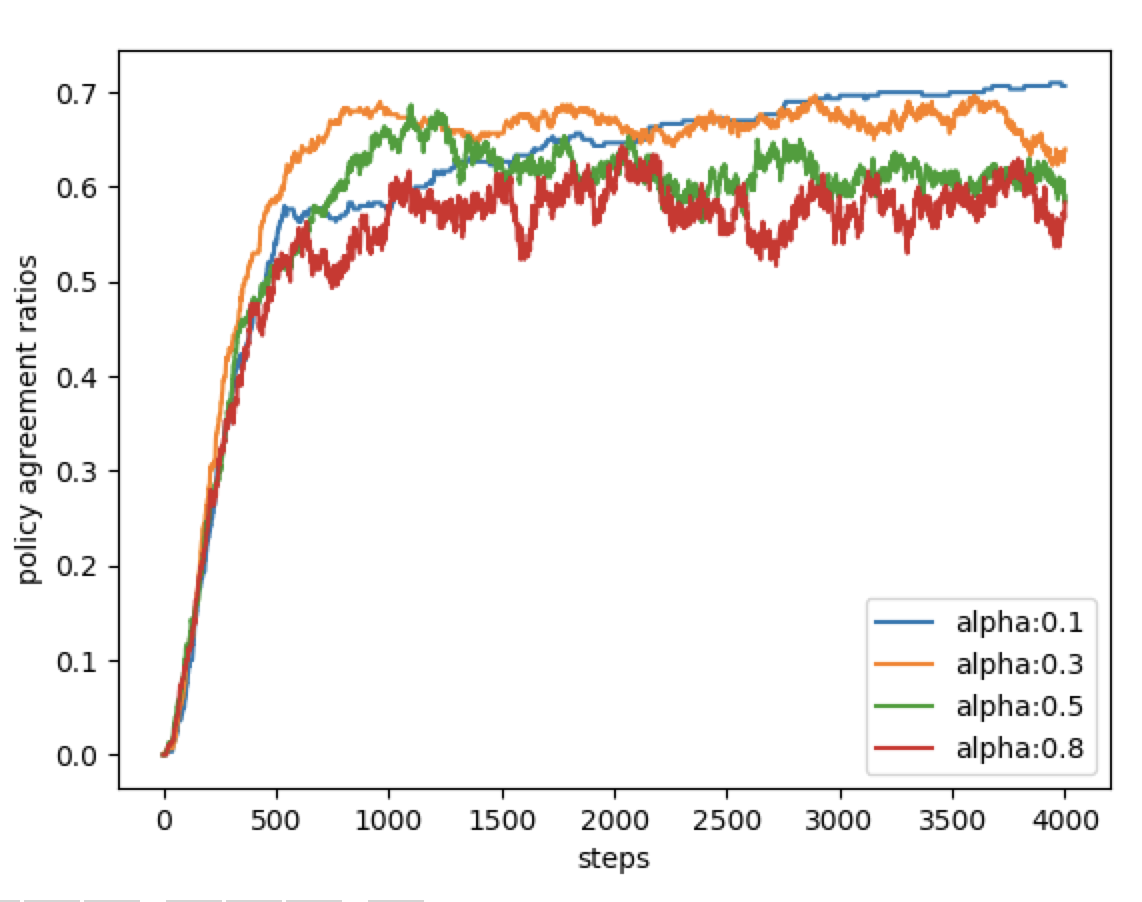
\includegraphics[width=0.9\linewidth, height=5cm]{images/alpha_noise02_4000.png}
		\caption{}
	\end{subfigure}
	\caption{Different Learning Rate with Noise 0.2 (Q-Learning)}
\end{figure}


\end{document}








